\documentclass[12pt, letterpaper]{../assignment}
\usepackage{graphicx}
\usepackage{courier}
\usepackage{minted}
\usepackage{amsmath}
\usepackage{polynom}
\usepackage{commath}
\usepackage{amssymb}
\usepackage{amsfonts} 
\usepackage{color}
\usepackage{cancel}
\usepackage{enumitem}
\usepackage{graphicx}
\usepackage{multirow}
\usepackage{float}
\usepackage{bm}
\usepackage{tikz}
\usetikzlibrary{shapes,arrows}
\usepackage{booktabs}
\usetikzlibrary{patterns}

% Define Theme Colors
\definecolor{light-gray}{rgb}{0.2,0.2,0.2}
\definecolor{header-blue}{rgb}{0,0,0.7}
% \definecolor{header-blue}{rgb}{0.5137,0.8353,0.9176}
\definecolor{header-blue}{rgb}{0,0.8,0.95}
\definecolor{dark-gray}{rgb}{0.1,0.1,0.1}
\pagecolor{dark-gray}
\color{white}

\usemintedstyle{monokai}
\oddsidemargin = 0pt
\exercisesheet{Module 7}{Assignment}
\student{Austin Barrilleaux}
\university{\color{header-blue}Johns Hopkins University}
\school{\color{header-blue}Whiting School of Engineering}
\courselabel{EN 535.612}
\semester{Fall 2024}
\usepackage[backend=bibtex,style=numeric,sorting=none]{biblatex}
\bibliography{reference}

\definecolor{light-gray}{rgb}{0.2,0.2,0.2}
\setminted{bgcolor=light-gray,frame=lines,rulecolor=white}
\setlength{\parindent}{0pt}

\makeatletter
\patchcmd{\minted@colorbg}{\noindent}{\medskip\noindent}{}{}
\apptocmd{\endminted@colorbg}{\par\medskip}{}{}
\makeatother

\begin{document}

\subsection*{EXERCISE 7.1}
\subsubsection*{The slider descends along a curved guide as
the guide translates to the right at the constant speed $\bm{u}$.
The shape of the guide bar in terms of a body-fixed set of coordinates is $\bm{y = \beta x^2}$.
Generalized coordinates selected for this system are the fixed X and Y coordinates of the collar.
Independently derive the velocity and configuration constraint equations relating X and Y.
Then show that integration of the velocity constraint yields the configuration constraint.}

\begin{figure}[H]
    \centering
    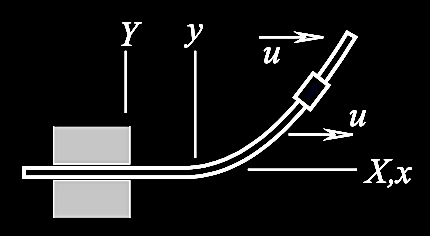
\includegraphics[scale=0.9,frame]{images/Q7_1.png}
\end{figure}



\subsection*{EXERCISE 7.12}
\subsubsection*{The figure shows a disk that is constrained to roll
without slipping on a horizontal XY plane,
such that its plane remains vertical.
Let the position coordinates X and Y of the geometric center,
the heading angle $\bm{\Psi}$,
and the spin angle $\bm{\phi}$ be generalized coordinates.
Describe the velocity constraints between these generalized coordinates.
From those results, determine the number of degrees of freedom,
and whether the system is holonomic.}

\begin{figure}[H]
    \centering
    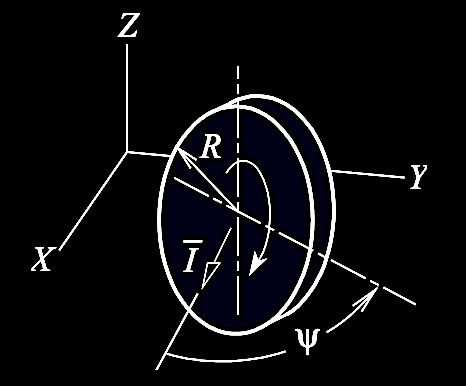
\includegraphics[scale=0.7,frame]{images/Q7_12.png}
\end{figure}



% % \color{white}
% \hspace*{6em}\inputminted[frame=leftline,fontsize=\footnotesize]{matlab}
% {./matlab/Q6_8.m}
% % \color{black} 

% \begin{figure}[H]
%     \centering
%     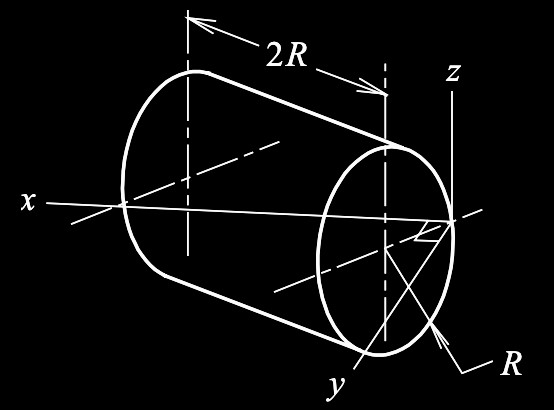
\includegraphics[scale=0.7,frame]{images/Q5_13.png}
% \end{figure}




\end{document}

